% Solid whose volume is given by  \int_0^1 \int_0^{1-x} \int_0^{2-2z} dy dz dx
% Region:  x>=0, y>=0, z>=0, x+z<=1, y+2z<=2
% => oblique rectangular pyramid, apex E=(0,0,1), base rectangle [0,1]x[0,2]x{0}
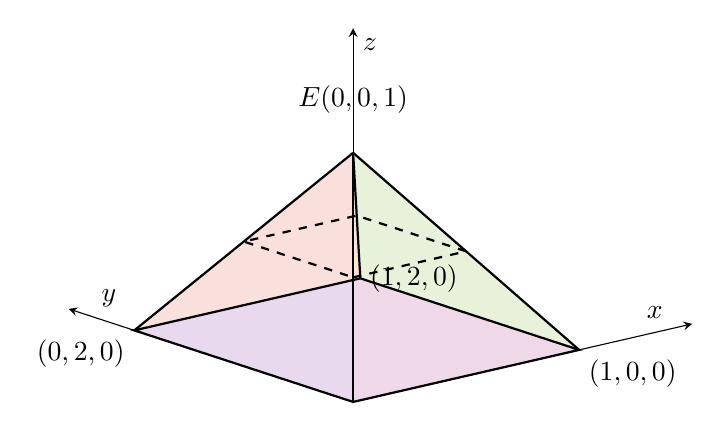
\begin{tikzpicture}
\begin{axis}[
    view={-40}{18},
    axis lines=center,
    axis line style={-stealth},
    xlabel={$x$}, ylabel={$y$}, zlabel={$z$},
    xmin=0, xmax=1.5,
    ymin=0, ymax=2.6,
    zmin=0, zmax=1.5,
    xtick=\empty, ytick=\empty, ztick=\empty,
    width=9.5cm, height=8.5cm,
    clip=false,
]
% ---- faces (filled, drawn back-to-front) ----
% base in z=0 : rectangle (0,0,0)-(1,0,0)-(1,2,0)-(0,2,0)
\addplot3[fill=blue!20, fill opacity=0.55, draw=none]
    coordinates {(0,0,0) (1,0,0) (1,2,0) (0,2,0) (0,0,0)};
% face y=0
\addplot3[fill=red!20, fill opacity=0.45, draw=none]
    coordinates {(0,0,1) (0,0,0) (1,0,0) (0,0,1)};
% face x+z=1
\addplot3[fill=green!20, fill opacity=0.45, draw=none]
    coordinates {(0,0,1) (1,0,0) (1,2,0) (0,0,1)};
% face y+2z=2
\addplot3[fill=orange!25, fill opacity=0.45, draw=none]
    coordinates {(0,0,1) (1,2,0) (0,2,0) (0,0,1)};
% face x=0
\addplot3[fill=purple!20, fill opacity=0.45, draw=none]
    coordinates {(0,0,1) (0,2,0) (0,0,0) (0,0,1)};

% ---- edges ----
\draw[thick] (axis cs:0,0,0) -- (axis cs:1,0,0) -- (axis cs:1,2,0)
             -- (axis cs:0,2,0) -- cycle;                       % base
\draw[thick] (axis cs:0,0,1) -- (axis cs:1,0,0);                % apex
\draw[thick] (axis cs:0,0,1) -- (axis cs:1,2,0);
\draw[thick] (axis cs:0,0,1) -- (axis cs:0,2,0);
\draw[thick] (axis cs:0,0,1) -- (axis cs:0,0,0);

% ---- labels ----
\node[above] at (axis cs:0,0,1.12) {$E(0,0,1)$};
\node[below right] at (axis cs:1,0,0) {$(1,0,0)$};
\node[below left]  at (axis cs:0,2,0) {$(0,2,0)$};
\node[right]       at (axis cs:1,2,0) {$(1,2,0)$};

% ---- a horizontal slice at z=1/2 : rectangle [0,1/2]x[0,1] ----
\addplot3[draw=black, dashed, thick]
    coordinates {(0,0,0.5) (0.5,0,0.5) (0.5,1,0.5) (0,1,0.5) (0,0,0.5)};
\end{axis}
\end{tikzpicture}
